% !TEX encoding = UTF-8 Unicode
% !TEX program = pdflatex
\documentclass[11pt,a4paper,twocolumn]{article}

%%% ---- packages ----
\usepackage[utf8]{inputenc}
\usepackage[T1]{fontenc}
\usepackage{times}
\usepackage{geometry}
\geometry{left=2cm,right=2cm,top=2.5cm,bottom=2.5cm}
\usepackage{graphicx}
\usepackage{booktabs}
\usepackage{amsmath,amssymb}
\usepackage{hyperref}
\usepackage{cleveref}
\usepackage{multirow}
\usepackage{array}
\usepackage{caption}
\usepackage{subcaption}
\usepackage{xcolor}
\usepackage{enumitem}
\usepackage{url}
\usepackage{balance}
\usepackage{float}
\usepackage{tikz}
\usetikzlibrary{shapes.geometric, arrows.meta, positioning, fit, calc, backgrounds, matrix}
\graphicspath{{figures/}}

\hypersetup{
  colorlinks=true,
  linkcolor=blue!60!black,
  citecolor=blue!60!black,
  urlcolor=blue!60!black
}

%%% ---- title ----
\title{Chunking and Embedding Strategies for Turkish Legal\\
Retrieval-Augmented Generation:\\
An Empirical Study on KVKK Corpus}

\author{
  Yamaç Demirkan Yılmaz\\
  Department of Computer Engineering\\
  \texttt{yamac@example.edu.tr}
}

\date{}

\begin{document}
\maketitle

%%% ====================================================================
%%% ABSTRACT
%%% ====================================================================
\begin{abstract}
Retrieval-Augmented Generation (RAG) is now the main way to connect large language models with real documents. However, most of the research about how to build these systems comes from English texts. This creates two problems for Turkish legal text. First, Turkish is an agglutinative language, which means words change their form a lot. This makes keyword matching harder and also affects how embedding models handle the text. Second, legal documents have a strict structure (articles, paragraphs, sub-paragraphs) and if you cut the text in the wrong place, you can change the legal meaning completely.

In this study, we test how different chunking methods, embedding models, and retrieval modes work together on a Turkish data protection law corpus. The corpus contains the full text of Law No.~6698 (KVKK), its regulations, and the decisions of the Turkish Data Protection Board --- 372 documents in total. We use a 35-question gold set where each question has an expert-verified source annotation, and we measure Recall@$k$, MRR, and nDCG.

We report three main findings. First, we find a silent truncation problem in a popular Turkish sentence embedding model. Second, we show that structure-aware chunking gives 45\% better MRR than fixed-length chunking on legal text. Third, we show that hybrid retrieval is not always better than dense-only retrieval --- it depends on how strong the dense encoder is. Additionally, we introduce authority weighting and cross-encoder reranking, which together raise the system from R@10\,=\,0.54 to R@10\,=\,0.77.
\end{abstract}

\textbf{Keywords:} retrieval-augmented generation, Turkish NLP, legal text, chunking, embedding, hybrid retrieval, cross-encoder reranking, KVKK

%%% ====================================================================
%%% 1. INTRODUCTION
%%% ====================================================================
\section{Introduction}
\label{sec:intro}

\subsection{Problem Setting}

A compliance assistant for Turkish data protection law needs to answer two very different types of questions:

\begin{enumerate}[leftmargin=*]
  \item \textbf{Conceptual queries} that are asked in everyday language. For example: ``Can I install a fingerprint reader at the office entrance?'' The law talks about \textit{biyometrik veri} (biometric data), but the user says \textit{parmak izi} (fingerprint). The words are completely different.
  \item \textbf{Referential queries} that mention a specific identifier. For example: ``What does Board Decision 2025/1072 say?'' Here, exact word matching is enough.
\end{enumerate}

These two query types need opposite things from the retrieval system. Conceptual queries need the system to understand meaning. Referential queries need the system to find exact tokens. If you optimize for one type, you will fail on the other. This is the main reason we use a hybrid architecture and why we report results separately for each query type.

\subsection{Why Legal Text is Different from General Text}

Turkish laws follow a strict hierarchy: \texttt{BÖLÜM} (chapter) $\rightarrow$ \texttt{MADDE} (article) $\rightarrow$ numbered paragraph $\rightarrow$ lettered sub-paragraph. The article is what lawyers actually cite. They say ``Article~5(2)(ç),'' not ``characters 4,300 to 5,300.''

When a fixed-length text splitter cuts across an article boundary, the retrieved piece might show a condition for lawful processing but without the clause that qualifies it. The result is an answer that sounds correct but is actually wrong. This is a very dangerous failure mode for a legal system.

\subsection{Contributions}

The contributions of this paper are:

\begin{itemize}[leftmargin=*]
  \item A reproducible, containerized Turkish legal RAG corpus and evaluation harness with 372 source documents and a 35-question gold set with verified source annotations.
  \item Finding and measuring a sequence-length truncation defect in a widely used Turkish sentence embedding model, which has a real effect on retrieval quality.
  \item A fully crossed comparison of 3 chunking strategies $\times$ 3 embedding configurations $\times$ 3 retrieval modes (27~configurations), measured with Recall@\{1,3,5,10\}, MRR, and nDCG, separated by query type.
  \item Introduction of authority weighting and cross-encoder reranking with analysis of their interaction, reaching R@10\,=\,0.77 and MRR\,=\,0.657 on the gold set.
\end{itemize}

Figure~\ref{fig:architecture} illustrates the end-to-end experimental RAG pipeline, spanning structure-aware chunking, dual-representation indexing, hybrid retrieval with authority weighting, cross-encoder reranking, and grounded generation with a local LLM.

\begin{figure*}[t]
\centering
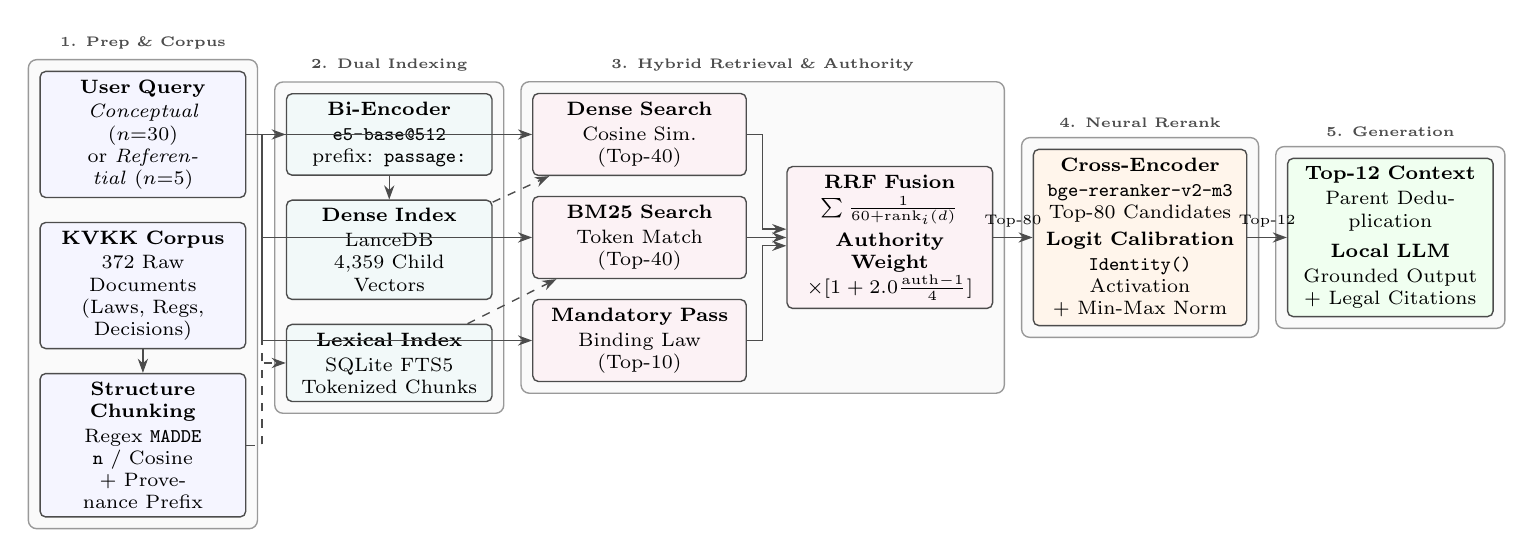
\begin{tikzpicture}[
  box/.style={draw=black!70, line width=0.5pt, rounded corners=2pt, align=center, font=\scriptsize, inner sep=3pt},
  stage/.style={draw=black!40, line width=0.5pt, fill=black!2, rounded corners=3pt, inner sep=4pt},
  proc/.style={box, fill=blue!4},
  idx/.style={box, fill=teal!5},
  ret/.style={box, fill=purple!5},
  rer/.style={box, fill=orange!8},
  gen/.style={box, fill=green!6},
  arrow/.style={-{Stealth[length=1.8mm, width=1.3mm]}, line width=0.5pt, draw=black!70},
  darrow/.style={arrow, dashed}
]

  % Stage 1: Preparation
  \node[proc, text width=2.4cm] (query) {\textbf{User Query}\\[1pt]\textit{Conceptual} ($n{=}30$)\\or \textit{Referential} ($n{=}5$)};
  \node[proc, text width=2.4cm, below=0.3cm of query] (corpus) {\textbf{KVKK Corpus}\\[1pt]372 Raw Documents\\(Laws, Regs, Decisions)};
  \node[proc, text width=2.4cm, below=0.3cm of corpus] (chunk) {\textbf{Structure Chunking}\\[1pt]Regex \texttt{MADDE n} / Cosine\\+ Provenance Prefix};
  \draw[arrow] (corpus) -- (chunk);

  % Stage 2: Dual Indexing
  \node[idx, text width=2.4cm, right=0.5cm of query] (enc) {\textbf{Bi-Encoder}\\[1pt]\texttt{e5-base@512}\\prefix: \texttt{passage:}};
  \node[idx, text width=2.4cm, below=0.3cm of enc] (dense) {\textbf{Dense Index}\\[1pt]LanceDB\\4,359 Child Vectors};
  \node[idx, text width=2.4cm, below=0.3cm of dense] (bm25) {\textbf{Lexical Index}\\[1pt]SQLite FTS5\\Tokenized Chunks};
  \draw[darrow] (chunk.east) -- ++(0.2,0) |- (enc.west);
  \draw[arrow] (enc) -- (dense);
  \draw[darrow] (chunk.east) -- ++(0.2,0) |- (bm25.west);

  % Stage 3: Hybrid Retrieval
  \node[ret, text width=2.5cm, right=0.5cm of enc] (search_dense) {\textbf{Dense Search}\\[1pt]Cosine Sim.\ (Top-40)};
  \node[ret, text width=2.5cm, below=0.25cm of search_dense] (search_bm25) {\textbf{BM25 Search}\\[1pt]Token Match (Top-40)};
  \node[ret, text width=2.5cm, below=0.25cm of search_bm25] (search_mand) {\textbf{Mandatory Pass}\\[1pt]Binding Law (Top-10)};
  \draw[arrow] (query.east) -- ++(0.2,0) |- (search_dense.west);
  \draw[arrow] (query.east) -- ++(0.2,0) |- (search_bm25.west);
  \draw[arrow] (query.east) -- ++(0.2,0) |- (search_mand.west);
  \draw[darrow] (dense) -- (search_dense);
  \draw[darrow] (bm25) -- (search_bm25);

  % Stage 4: Fusion & Calibration
  \node[ret, text width=2.4cm, right=0.5cm of search_bm25] (fusion) {\textbf{RRF Fusion}\\[1pt]$\sum \frac{1}{60 + \text{rank}_i(d)}$\\[2pt]\textbf{Authority Weight}\\[1pt]$\times [1 + 2.0\frac{\text{auth}-1}{4}]$};
  \draw[arrow] (search_dense.east) -- ++(0.2,0) |- ([yshift=3pt]fusion.west);
  \draw[arrow] (search_bm25.east) -- (fusion.west);
  \draw[arrow] (search_mand.east) -- ++(0.2,0) |- ([yshift=-3pt]fusion.west);

  % Stage 5: Cross-Encoder Reranking
  \node[rer, text width=2.5cm, right=0.5cm of fusion] (rerank) {\textbf{Cross-Encoder}\\[1pt]\texttt{bge-reranker-v2-m3}\\Top-80 Candidates\\[2pt]\textbf{Logit Calibration}\\[1pt]\texttt{Identity()} Activation\\+ Min-Max Norm};
  \draw[arrow] (fusion) -- node[above, font=\tiny]{Top-80} (rerank);

  % Stage 6: Generation
  \node[gen, text width=2.4cm, right=0.5cm of rerank] (gen) {\textbf{Top-12 Context}\\[1pt]Parent Deduplication\\[3pt]\textbf{Local LLM}\\[1pt]Grounded Output\\+ Legal Citations};
  \draw[arrow] (rerank) -- node[above, font=\tiny]{Top-12} (gen);

  % Grouping backgrounds
  \begin{scope}[on background layer]
    \node[stage, fit=(query)(corpus)(chunk), label={[font=\tiny\bfseries, text=black!70]above:1. Prep \& Corpus}] {};
    \node[stage, fit=(enc)(dense)(bm25), label={[font=\tiny\bfseries, text=black!70]above:2. Dual Indexing}] {};
    \node[stage, fit=(search_dense)(search_bm25)(search_mand)(fusion), label={[font=\tiny\bfseries, text=black!70]above:3. Hybrid Retrieval \& Authority}] {};
    \node[stage, fit=(rerank), label={[font=\tiny\bfseries, text=black!70]above:4. Neural Rerank}] {};
    \node[stage, fit=(gen), label={[font=\tiny\bfseries, text=black!70]above:5. Generation}] {};
  \end{scope}

\end{tikzpicture}
\caption{End-to-end experimental RAG architecture. 372 raw legal documents are partitioned via structure-aware chunking and dual-indexed into LanceDB (dense) and SQLite FTS5 (BM25). The hybrid retriever combines dense, lexical, and mandatory binding-source candidates via RRF ($k{=}60$), applies authority calibration ($w{=}2.0$), and forwards the top-80 candidates to a cross-encoder for final reranking and deduplication before grounded answer generation with a local LLM.}
\label{fig:architecture}
\end{figure*}


%%% ====================================================================
%%% 2. RELATED WORK
%%% ====================================================================
\section{Related Work}
\label{sec:related}

\subsection{Chunking Strategy}

Qu et al.~\cite{qu2025} question whether semantic chunking is worth the cost. They find that fixed-size chunking consistently outperforms semantic chunking across document retrieval, evidence retrieval, and answer generation. They conclude that the extra computation for semantic chunking does not give consistent improvements. This finding is the main null hypothesis we test in our study.

In the legal domain, researchers from Vrije Universiteit Brussel~\cite{jurix2024} tested three chunking methods (simple text splitting, recursive text splitting, and semantic chunking) on the GDPR. They scored 17 legal questions by cosine similarity and found that no method consistently produced high semantic relevance at the individual chunk level. This motivated our decision to use rank-based IR metrics instead of chunk-level cosine similarity.

Our structure-aware approach is different from both of these: instead of guessing where the boundaries should be, we parse the legislative hierarchy directly and use the article as the retrieval unit.

\subsection{Turkish RAG}

Ünlü et al.~\cite{ragturk2026} (RAGTurk, SIGTURK 2026) benchmark seven stages of the RAG pipeline on Turkish data. They report that HyDE gives the best accuracy (85.0\%), but cross-encoder reranking plus context augmentation achieves very close results (84.6\%) at much lower cost. Very importantly for our design, they find that stacking too many generative modules actually makes things worse because it distorts the morphological features of Turkish. We therefore use reranking as the main improvement and do not stack generative rewriting stages.

Türkel et al.~\cite{turkel2026} compare three chunking strategies, five embedding models, and two generator LLMs across documents with different layouts. Their fully crossed experimental design is the methodological template for our study. We use the same crossed structure but substitute a legal corpus and retrieval-level metrics.

\subsection{Legal RAG and Grounding}

Abualhaija et al.~\cite{abualhaija2025} use LLMs with RAG to extract GDPR requirements. They achieve 81.8\% and 85.7\% correctness, but only 68.2\% and 50.0\% of the generated legal references were properly grounded. This means the model often cites the main article but forgets the related provisions. This motivates two of our design decisions: a mandatory-source quota and forced inclusion of sibling paragraphs.

\subsection{Context Enrichment}

Two recent methods try to solve the problem that a chunk loses its document context when embedded alone. \textit{Late Chunking}~\cite{gunther2024} embeds the entire document first and then creates chunk vectors from the token representations. \textit{Contextual Retrieval}~\cite{anthropic2024} adds a short description of where the chunk comes from before embedding it.

We implement a simple, deterministic version of contextual retrieval: each chunk gets a provenance prefix like \texttt{[Law 6698 · Art.~5 --- Conditions for processing]}. In Section~\ref{sec:discussion} we show why this prefix has a dangerous interaction with a truncating encoder.


%%% ====================================================================
%%% 3. CORPUS
%%% ====================================================================
\section{Corpus}
\label{sec:corpus}

We collected the corpus from the official website of the Turkish Personal Data Protection Authority (kvkk.gov.tr), the consolidated text of Law No.~6698 from mevzuat.gov.tr, and two regulations from the Official Gazette.

\begin{table}[t]
\centering
\caption{Corpus composition by source type. Authority scores are used in the authority weighting mechanism (Section~\ref{subsec:authority}).}
\label{tab:corpus}
\small
\begin{tabular}{@{}lccr@{}}
\toprule
\textbf{Source type} & \textbf{Binding} & \textbf{Auth.} & \textbf{Docs} \\
\midrule
Law No. 6698        & mandatory & 5 & 1 \\
Regulations         & mandatory & 4 & 8 \\
Communiqués         & mandatory & 4 & 3 \\
Principle decisions & mandatory & 4 & 8 \\
Board decisions     & mandatory & 3 & 21 \\
Decision summaries  & advisory  & 2 & 314 \\
Standard clauses    & mandatory & 3 & 8 \\
Guidance pages      & advisory  & 1 & 2 \\
\midrule
\textbf{Total}      &           &   & \textbf{365} \\
\bottomrule
\end{tabular}
\end{table}

Table~\ref{tab:corpus} shows the corpus composition. The binding/advisory distinction follows the separation used by Abualhaija et al.~\cite{abualhaija2025}. An important thing to notice is the class imbalance: decision summaries are 87\% of documents by count but they have the second-lowest authority weight. This imbalance directly motivates the mandatory-source mechanism we describe in Section~\ref{subsec:authority}.

We excluded 10 scanned image-only PDFs (no text layer), 2 JavaScript shell pages with no content, and 2 byte-identical duplicates. All exclusions were logged with reasons.


%%% ====================================================================
%%% 4. METHOD
%%% ====================================================================
\section{Method}
\label{sec:method}

\subsection{Experimental Design}

We use a fully crossed design with three factors, as shown in Table~\ref{tab:factors}. This gives us $3 \times 3 \times 3 = 27$ configurations, each evaluated on the same 35-question gold set.

\begin{table}[t]
\centering
\caption{Experimental factors and their levels.}
\label{tab:factors}
\small
\begin{tabular}{@{}ll@{}}
\toprule
\textbf{Factor} & \textbf{Levels} \\
\midrule
Chunking   & \texttt{recursive} (1000 chars, 200 overlap) \\
           & \texttt{recursive+prefix} \\
           & \texttt{structural+semantic} \\
\midrule
Embedding  & \texttt{berturk-sts@75} \\
           & \texttt{berturk-sts@512} \\
           & \texttt{e5-base@512} \\
\midrule
Retrieval  & \texttt{dense} \\
           & \texttt{bm25} \\
           & \texttt{hybrid} (RRF, $k{=}60$) \\
\bottomrule
\end{tabular}
\end{table}

The \texttt{recursive+prefix} condition has exactly the same text boundaries as \texttt{recursive}. The only difference is the provenance prefix. This lets us measure the prefix effect separately from the boundary effect.

\subsection{Chunking Conditions}

\textbf{Recursive (baseline).} Fixed 1000-character windows with 200-character overlap, splitting on \texttt{\textbackslash n\textbackslash n} $\rightarrow$ \texttt{\textbackslash n} $\rightarrow$ \texttt{. } $\rightarrow$ \texttt{ } in priority order. This is the default configuration used by most RAG systems and matches the ``Recursive'' arm in the JURIX study~\cite{jurix2024}.

\textbf{Structural + semantic (proposed).} We route the chunking by document type:

\begin{itemize}[leftmargin=*]
  \item \textit{Legislation} --- we parse on the article marker regex \texttt{MADDE~n}, which works for both old and new Official Gazette formatting styles. Parent = article; child = numbered paragraph. Article headings are recovered from the preceding line.
  \item \textit{Decisions and guidance} --- these have no article structure, so we use a different approach. We merge paragraphs to a ${\sim}$700-character target and place boundaries where the cosine similarity between consecutive units falls below the 5th percentile of that document's similarity distribution. We also enforce a hard maximum of 1300 characters.
\end{itemize}

Figure~\ref{fig:chunking} illustrates how the two chunking strategies differ. The recursive baseline applies a fixed-length window to all documents, while the structural+semantic approach routes documents by type and uses explicit article markers for legislation.

\begin{figure}[t]
\centering
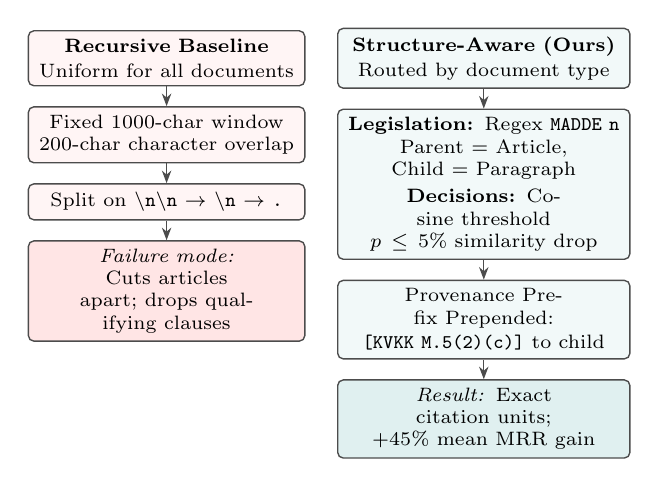
\begin{tikzpicture}[
  box/.style={draw=black!70, line width=0.5pt, rounded corners=2pt, align=center, font=\scriptsize, inner sep=3pt},
  base/.style={box, fill=red!4, text width=3.3cm},
  prop/.style={box, fill=teal!5, text width=3.5cm},
  arrow/.style={-{Stealth[length=1.6mm, width=1.2mm]}, line width=0.5pt, draw=black!70}
]

  % Baseline (Left)
  \node[base] (r_in) {\textbf{Recursive Baseline}\\[1pt]Uniform for all documents};
  \node[base, below=0.25cm of r_in] (r_win) {Fixed 1000-char window\\200-char character overlap};
  \node[base, below=0.25cm of r_win] (r_split) {Split on \texttt{\textbackslash n\textbackslash n} $\rightarrow$ \texttt{\textbackslash n} $\rightarrow$ \texttt{. }};
  \node[base, fill=red!10, below=0.25cm of r_split] (r_out) {\textit{Failure mode:} Cuts articles\\apart; drops qualifying clauses};
  \draw[arrow] (r_in) -- (r_win);
  \draw[arrow] (r_win) -- (r_split);
  \draw[arrow] (r_split) -- (r_out);

  % Proposed (Right)
  \node[prop, right=0.4cm of r_in] (s_in) {\textbf{Structure-Aware (Ours)}\\[1pt]Routed by document type};
  \node[prop, below=0.25cm of s_in] (s_route) {\textbf{Legislation:} Regex \texttt{MADDE n}\\Parent = Article, Child = Paragraph\\[2pt]\textbf{Decisions:} Cosine threshold\\$p \le 5\%$ similarity drop};
  \node[prop, below=0.25cm of s_route] (s_pref) {Provenance Prefix Prepended:\\[1pt]\texttt{[KVKK M.5(2)(c)]} to child};
  \node[prop, fill=teal!12, below=0.25cm of s_pref] (s_out) {\textit{Result:} Exact citation units;\\+45\% mean MRR gain};
  \draw[arrow] (s_in) -- (s_route);
  \draw[arrow] (s_route) -- (s_pref);
  \draw[arrow] (s_pref) -- (s_out);

\end{tikzpicture}
\caption{Chunking strategy comparison. The recursive baseline blindly cuts text by character count, often separating qualifications from rules. The proposed approach routes legislation through article-marker regex and decisions through cosine similarity breakpoints, adding a provenance prefix to every child.}
\label{fig:chunking}
\end{figure}

\subsection{Embedding Conditions}

\texttt{emrecan/bert-base-turkish-cased-mean-nli-stsb-tr} (which we call ``BERTurk-STS'') is a BERTurk backbone fine-tuned on Turkish NLI/STS data. It is a common default choice for Turkish semantic search. We test it at its shipped \texttt{max\_seq\_length} of 75 tokens and at 512 tokens (the BERT positional limit).

\texttt{intfloat/multilingual-e5-base} (``E5-base'') is trained natively at 512 tokens. We evaluate it with the required asymmetric \texttt{query:} / \texttt{passage:} prefixes.

\subsection{Retrieval and Scoring}
\label{subsec:retrieval}

Only child chunks are embedded. When we retrieve children, we map them to their parent, remove duplicates, and return the parent as the retrieval unit. This means the unit we evaluate is the complete article or decision --- the thing a practitioner would actually cite.

For hybrid retrieval, we fuse the dense and lexical rankings with Reciprocal Rank Fusion (RRF):
\begin{equation}
  \text{score}(d) = \sum_i \frac{1}{k + \text{rank}_i(d)}, \quad k = 60
  \label{eq:rrf}
\end{equation}

A retrieved parent counts as a hit if every field in the gold annotation matches (source type, article number, decision number, or document-name substring). We report Recall@\{1,3,5,10\}, MRR, and nDCG.

Figure~\ref{fig:retrieval} shows the detailed retrieval pipeline, including both the main and mandatory passes, the RRF fusion, authority weighting, and cross-encoder reranking stages.

\begin{figure*}[t]
\centering
\begin{tikzpicture}[
  box/.style={draw=black!70, line width=0.5pt, rounded corners=2pt, align=center, font=\scriptsize, inner sep=3.5pt},
  flow/.style={box, fill=purple!5, text width=2.7cm},
  fuse/.style={box, fill=blue!5, text width=3.6cm},
  score/.style={box, fill=orange!8, text width=3.8cm},
  out/.style={box, fill=teal!6, text width=3.2cm},
  arrow/.style={-{Stealth[length=1.8mm, width=1.3mm]}, line width=0.5pt, draw=black!70}
]

  % Inputs
  \node[flow] (q) {\textbf{User Query $q$}\\[2pt]\texttt{query: <metin>}};
  \node[flow, right=0.6cm of q] (enc) {\textbf{Bi-Encoder}\\[2pt]\texttt{e5-base @512}\\[1pt]768-dim query vector};
  \draw[arrow] (q) -- (enc);

  % Parallel channels
  \node[flow, right=0.7cm of enc] (dense) {\textbf{Dense Search}\\[1pt]LanceDB (Cosine)\\[1pt]Top-40 Children $\rightarrow$ Dedup};
  \node[flow, above=0.3cm of dense] (bm25) {\textbf{Lexical Search}\\[1pt]SQLite FTS5 (BM25)\\[1pt]Top-40 Children $\rightarrow$ Dedup};
  \node[flow, below=0.3cm of dense] (mand) {\textbf{Mandatory Pass}\\[1pt]\texttt{binding = 'zorunlu'}\\[1pt]Top-10 Binding Parents};

  \draw[arrow] (enc.east) -- ++(0.3,0) |- (bm25.west);
  \draw[arrow] (enc.east) -- (dense.west);
  \draw[arrow] (enc.east) -- ++(0.3,0) |- (mand.west);

  % RRF Fusion
  \node[fuse, right=0.7cm of dense] (rrf) {\textbf{Reciprocal Rank Fusion}\\[2pt]$S_{\text{rrf}}(d) = \sum_{i} \frac{1}{60 + \text{rank}_i(d)}$\\[2pt]$i \in \{\text{dense}, \text{bm25}, \text{mandatory}\}$};
  \draw[arrow] (bm25.east) -- ++(0.3,0) |- ([yshift=4pt]rrf.west);
  \draw[arrow] (dense.east) -- (rrf.west);
  \draw[arrow] (mand.east) -- ++(0.3,0) |- ([yshift=-4pt]rrf.west);

  % Authority Weighting
  \node[score, right=0.7cm of rrf] (auth) {\textbf{Authority Calibration ($w{=}2.0$)}\\[2pt]$S_{\text{cal}}(d) = S_{\text{rrf}}(d) \times \left[1 + 2.0 \cdot \frac{\text{auth}(d) - 1}{4}\right]$\\[2pt]\textit{Law}${=}5, \dots, \textit{Guidance}${=}2, \textit{Summary}${=}1$};
  \draw[arrow] (rrf) -- (auth);

  % Cross-Encoder & Output
  \node[out, right=0.7cm of auth] (ce) {\textbf{Neural Reranking}\\[2pt]\texttt{bge-reranker-v2-m3}\\[1pt]Top-80 Candidates $\rightarrow$\\[1pt]$\text{MinMax}(\text{Logits})$\\[2pt]\textbf{Final Top-12 Parents}\\(R@10=0.77, MRR=0.657)};
  \draw[arrow] (auth) -- node[above, font=\tiny]{Top-80} (ce);

\end{tikzpicture}
\caption{Detailed multi-stage retrieval and scoring pipeline. Parallel dense, lexical, and mandatory binding passes are merged via Reciprocal Rank Fusion ($k{=}60$), calibrated with statutory authority multipliers ($w{=}2.0$), and finally reranked by a cross-encoder using normalized raw logits to produce the top-12 context parents.}
\label{fig:retrieval}
\end{figure*}

\subsection{Authority Weighting and Mandatory-Source Retrieval}
\label{subsec:authority}

Two mechanisms were added to the production retriever and tested on the same gold set, but they are not part of the 27-configuration experiment matrix.

\textbf{Authority weighting} multiplies the fused score by:
\begin{equation}
  1 + w \cdot \frac{\text{authority} - 1}{4}
  \label{eq:auth}
\end{equation}
where $w$ is the authority weight parameter and authority values come from Table~\ref{tab:corpus}.

\textbf{Mandatory-source retrieval} runs a second retrieval pass filtered by metadata (\texttt{baglayicilik LIKE 'zorunlu\%'}), which guarantees that binding law enters the candidate pool even if many decision summaries outrank it in pure similarity.

\subsection{Cross-Encoder Reranking}
\label{subsec:reranking}

To improve top-rank precision, we add a cross-encoder reranker (\texttt{BAAI/bge-reranker-v2-m3}) over the top-80 fused candidate parents. During implementation, we found and fixed a double-sigmoid defect (described in Section~\ref{subsec:sigmoid}).

\subsection{Gold Set}

35 questions: 30 conceptual (everyday phrasing, no identifier) and 5 referential (explicit article or decision number). Each question is graded easy, medium, or hard. Every gold annotation was verified to resolve against the ingested corpus before running the experiments.

\subsection{Reproducibility}

All experiments run inside a CUDA container (\texttt{pytorch/pytorch:2.5.1-cuda12.1-cudnn9-runtime}) on an NVIDIA RTX 4050 Laptop GPU (6~GB). The harness builds indices in memory (NumPy inner product for dense, \texttt{rank\_bm25} for lexical) independently of the production stores. The \texttt{recursive} arm was run twice in separate container invocations and produced bit-identical metrics, which confirms determinism.


%%% ====================================================================
%%% 5. RESULTS
%%% ====================================================================
\section{Results}
\label{sec:results}

\subsection{Full Results}

Table~\ref{tab:full} shows the results for all 27~configurations. The ``miss'' column shows how many of the 35 questions had no correct result in the top~10.

\begin{table*}[t]
\centering
\caption{Full results for all 27 configurations on the 35-question gold set. \textbf{Bold} marks the best value in each metric. $R@k$ = Recall@$k$; \textit{miss} = questions with no correct source in the top 10.}
\label{tab:full}
\small
\begin{tabular}{@{}llcccccr@{}}
\toprule
\textbf{Chunking} & \textbf{Embedding} & \textbf{Retrieval} & \textbf{R@1} & \textbf{R@5} & \textbf{R@10} & \textbf{MRR} & \textbf{miss} \\
\midrule
recursive           & berturk@75  & dense  & 0.03 & 0.11 & 0.17 & 0.078 & 29 \\
recursive           & berturk@75  & bm25   & 0.14 & 0.23 & 0.26 & 0.181 & 26 \\
recursive           & berturk@75  & hybrid & 0.09 & 0.23 & 0.23 & 0.145 & 27 \\
recursive           & berturk@512 & dense  & 0.03 & 0.14 & 0.23 & 0.088 & 27 \\
recursive           & berturk@512 & bm25   & 0.14 & 0.23 & 0.26 & 0.181 & 26 \\
recursive           & berturk@512 & hybrid & 0.14 & 0.26 & 0.26 & 0.183 & 26 \\
recursive           & e5-base     & dense  & 0.20 & 0.29 & 0.31 & 0.231 & 24 \\
recursive           & e5-base     & bm25   & 0.14 & 0.23 & 0.26 & 0.181 & 26 \\
recursive           & e5-base     & hybrid & 0.20 & 0.26 & 0.29 & 0.233 & 25 \\
\midrule
recursive+prefix    & berturk@75  & dense  & 0.14 & 0.17 & 0.23 & 0.156 & 27 \\
recursive+prefix    & berturk@75  & bm25   & 0.17 & 0.26 & 0.29 & 0.212 & 25 \\
recursive+prefix    & berturk@75  & hybrid & 0.11 & 0.26 & 0.31 & 0.175 & 24 \\
recursive+prefix    & berturk@512 & dense  & 0.09 & 0.23 & 0.29 & 0.134 & 25 \\
recursive+prefix    & berturk@512 & bm25   & 0.17 & 0.26 & 0.29 & 0.212 & 25 \\
recursive+prefix    & berturk@512 & hybrid & 0.14 & 0.26 & 0.34 & 0.190 & 23 \\
recursive+prefix    & e5-base     & dense  & 0.23 & 0.26 & 0.31 & 0.249 & 24 \\
recursive+prefix    & e5-base     & bm25   & 0.17 & 0.26 & 0.29 & 0.212 & 25 \\
recursive+prefix    & e5-base     & hybrid & 0.23 & 0.29 & 0.34 & 0.256 & 23 \\
\midrule
structural+semantic & berturk@75  & dense  & 0.09 & 0.26 & 0.46 & 0.172 & 19 \\
structural+semantic & berturk@75  & bm25   & 0.14 & 0.29 & 0.34 & 0.209 & 23 \\
structural+semantic & berturk@75  & hybrid & 0.23 & 0.37 & 0.49 & \textbf{0.305} & 18 \\
structural+semantic & berturk@512 & dense  & 0.14 & 0.29 & 0.40 & 0.209 & 21 \\
structural+semantic & berturk@512 & bm25   & 0.14 & 0.29 & 0.34 & 0.209 & 23 \\
structural+semantic & berturk@512 & hybrid & 0.17 & 0.31 & 0.43 & 0.247 & 20 \\
structural+semantic & e5-base     & dense  & \textbf{0.26} & \textbf{0.43} & 0.49 & 0.330 & 18 \\
structural+semantic & e5-base     & bm25   & 0.14 & 0.29 & 0.34 & 0.209 & 23 \\
structural+semantic & e5-base     & hybrid & 0.20 & 0.40 & \textbf{0.51} & 0.292 & \textbf{17} \\
\bottomrule
\end{tabular}
\end{table*}

The best configuration by R@10 is \texttt{structural+semantic} with \texttt{e5-base} and \texttt{hybrid} retrieval (R@10\,=\,0.51, 17 misses). The best by MRR is the same chunking with \texttt{berturk@75} and \texttt{hybrid} (MRR\,=\,0.305).

\subsection{Marginal Means}

To understand which factor matters most, we calculate the marginal mean MRR for each level by averaging over the nine configurations where it appears (Table~\ref{tab:marginal}).

\begin{table}[t]
\centering
\caption{Marginal mean MRR for each factor level.}
\label{tab:marginal}
\small
\begin{tabular}{@{}lr|lr|lr@{}}
\toprule
\textbf{Chunking} & \textbf{MRR} & \textbf{Embed.} & \textbf{MRR} & \textbf{Retr.} & \textbf{MRR} \\
\midrule
recursive   & .167 & berturk@75  & .181 & dense  & .183 \\
rec.+prefix & .200 & berturk@512 & .184 & bm25   & .201 \\
struct.+sem.& \textbf{.242} & e5-base     & \textbf{.244} & hybrid & \textbf{.225} \\
\midrule
\textit{rel. gain} & \textit{+45\%} & \textit{rel. gain} & \textit{+35\%} & \textit{rel. gain} & \textit{+23\%} \\
\bottomrule
\end{tabular}
\end{table}

The chunking strategy is the single largest factor (+45\%), ahead of the embedding model choice (+35\%) and retrieval mode (+23\%).

\subsection{Results by Query Type}

Table~\ref{tab:querytype} shows Recall@5 separated by query type. Dense retrieval alone scores 0.00 on referential queries under plain recursive chunking. This happens because the article number is metadata, not prose --- the embedding of the article body has no signal for a query like ``what does Article~12 regulate?''

\begin{table}[t]
\centering
\caption{Recall@5 by query type for selected configurations. Conceptual: $n{=}30$; Referential: $n{=}5$.}
\label{tab:querytype}
\small
\begin{tabular}{@{}llccc@{}}
\toprule
\textbf{Chunk} & \textbf{Embed.} & \textbf{Retr.} & \textbf{Conc.} & \textbf{Ref.} \\
\midrule
recursive    & bert@75  & dense  & 0.13 & \textbf{0.00} \\
recursive    & bert@512 & dense  & 0.17 & \textbf{0.00} \\
recursive    & e5-base  & dense  & 0.30 & 0.20 \\
rec.+prefix  & bert@75  & bm25   & 0.23 & 0.40 \\
rec.+prefix  & e5-base  & hybrid & 0.30 & 0.20 \\
struct.+sem. & bert@75  & hybrid & 0.33 & \textbf{0.60} \\
struct.+sem. & e5-base  & dense  & \textbf{0.47} & 0.20 \\
struct.+sem. & e5-base  & hybrid & 0.43 & 0.20 \\
\bottomrule
\end{tabular}
\end{table}

\subsection{Authority Weighting and Mandatory Pass}
\label{subsec:auth_results}

Table~\ref{tab:authority} shows the effect of authority weighting and the mandatory-source retrieval pass. These results use the best base configuration (\texttt{structural+semantic}, \texttt{e5-base}, \texttt{hybrid}).

\begin{table}[t]
\centering
\caption{Authority weighting ($w$) and mandatory-source pass on the gold set. ``Ungrnd.''\ = questions where the entire top-10 consists of advisory sources only.}
\label{tab:authority}
\small
\begin{tabular}{@{}ccccccr@{}}
\toprule
\textbf{Mand.} & $\boldsymbol{w}$ & \textbf{R@1} & \textbf{R@10} & \textbf{MRR} & \textbf{miss} & \textbf{Ung.} \\
\midrule
off    & 0.0 & 0.29 & 0.54 & 0.357 & 16 & --- \\
off    & 0.5 & 0.37 & 0.66 & 0.441 & 12 & 1 \\
off    & 1.0 & 0.40 & 0.69 & \textbf{0.464} & 11 & 1 \\
top-5  & 1.0 & 0.26 & 0.66 & 0.380 & 12 & \textbf{0} \\
top-10 & 1.0 & 0.26 & \textbf{0.71} & 0.380 & \textbf{10} & \textbf{0} \\
top-20 & 1.0 & 0.26 & 0.66 & 0.384 & 12 & \textbf{0} \\
\bottomrule
\end{tabular}
\end{table}

Authority weighting alone is the single largest improvement we measured in this study: MRR went from 0.357 to 0.464 (+30\%), R@10 from 0.54 to 0.69, and misses from 16 to 11. A sensitivity analysis over $w \in \{0, 0.3, 0.5, 0.8, 1.0, 1.3, 1.6, 2.0, 3.0\}$ showed that MRR keeps going up at $w{=}3.0$ (reaching 0.560), but R@10 and miss count were flat from $w{=}0.8$ onward (0.69 / 11). This means higher $w$ does not find new documents --- it just reorders the candidates in a way that matches the gold set's statute-heavy composition. We adopted $w{=}1.0$ as the saturation point, explicitly declining the higher MRR as gold-set overfitting.

The mandatory pass trades rank quality for coverage: MRR falls to 0.380 but R@10 rises to 0.71 and, most importantly, ungrounded questions reach zero.

\subsection{Cross-Encoder Reranking}
\label{subsec:sigmoid}

\subsubsection{Double-Sigmoid Defect}

During implementation of the cross-encoder, we found a subtle bug. The \texttt{sentence-transformers} library's \texttt{CrossEncoder.predict()} method already applies a sigmoid activation internally when \texttt{num\_labels\,=\,1}. We were applying a second sigmoid in our scoring pipeline. This compressed all logits into a narrow band around ${\sim}0.50$, which basically destroyed the cross-encoder's ability to distinguish between candidates.

Paradoxically, this broken configuration produced better metrics (R@5\,=\,0.77, MRR\,=\,0.657, 8~misses at $w{=}1.0$) because the near-constant CE scores allowed the authority multiplier to act as the sole ranking signal --- which works well on a statute-heavy gold set.

We fixed the defect by extracting raw logits via \texttt{activation\_fct=torch.nn.Identity()} and applying candidate-set min-max normalization. However, restoring genuine cross-encoder variance diluted the authority signal at $w{=}1.0$, temporarily dropping recall.

Figure~\ref{fig:sigmoid} visualizes the defect and its fix.

\begin{figure}[t]
\centering
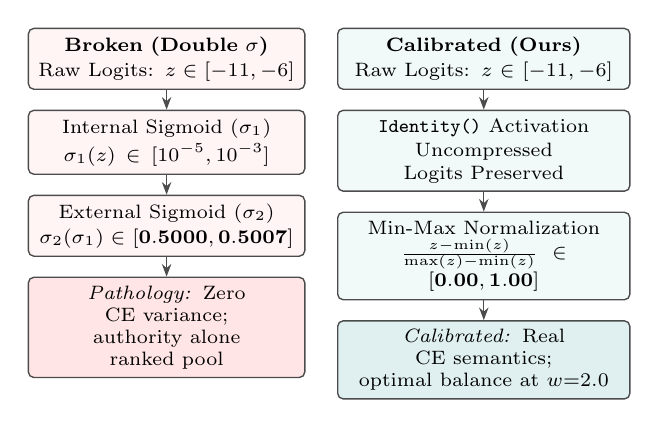
\begin{tikzpicture}[
  box/.style={draw=black!70, line width=0.5pt, rounded corners=2pt, align=center, font=\scriptsize, inner sep=3pt},
  broken/.style={box, fill=red!4, text width=3.3cm},
  fixed/.style={box, fill=teal!5, text width=3.5cm},
  arrow/.style={-{Stealth[length=1.6mm, width=1.2mm]}, line width=0.5pt, draw=black!70}
]

  % Broken (Left)
  \node[broken] (b_in) {\textbf{Broken (Double $\sigma$)}\\[1pt]Raw Logits: $z \in [-11, -6]$};
  \node[broken, below=0.25cm of b_in] (b_s1) {Internal Sigmoid ($\sigma_1$)\\[1pt]$\sigma_1(z) \in [10^{-5}, 10^{-3}]$};
  \node[broken, below=0.25cm of b_s1] (b_s2) {External Sigmoid ($\sigma_2$)\\[1pt]$\sigma_2(\sigma_1) \in \mathbf{[0.5000, 0.5007]}$};
  \node[broken, fill=red!10, below=0.25cm of b_s2] (b_out) {\textit{Pathology:} Zero CE variance;\\authority alone ranked pool};
  \draw[arrow] (b_in) -- (b_s1);
  \draw[arrow] (b_s1) -- (b_s2);
  \draw[arrow] (b_s2) -- (b_out);

  % Fixed (Right)
  \node[fixed, right=0.4cm of b_in] (f_in) {\textbf{Calibrated (Ours)}\\[1pt]Raw Logits: $z \in [-11, -6]$};
  \node[fixed, below=0.25cm of f_in] (f_id) {\texttt{Identity()} Activation\\[1pt]Uncompressed Logits Preserved};
  \node[fixed, below=0.25cm of f_id] (f_norm) {Min-Max Normalization\\[1pt]$\frac{z - \min(z)}{\max(z) - \min(z)} \in \mathbf{[0.00, 1.00]}$};
  \node[fixed, fill=teal!12, below=0.25cm of f_norm] (f_out) {\textit{Calibrated:} Real CE semantics;\\optimal balance at $w{=}2.0$};
  \draw[arrow] (f_in) -- (f_id);
  \draw[arrow] (f_id) -- (f_norm);
  \draw[arrow] (f_norm) -- (f_out);

\end{tikzpicture}
\caption{Double-sigmoid defect and calibration. \textbf{Left:} Applying sigmoid twice compressed cross-encoder logits into a degenerate range around $0.50$, destroying neural ranking. \textbf{Right:} Bypassing internal activation via \texttt{Identity()} and min-max normalizing restored the full $[0,1]$ range, requiring authority recalibration ($w{=}2.0$).}
\label{fig:sigmoid}
\end{figure}

\subsubsection{Authority Weight Recalibration}

A sensitivity sweep over $w \in \{1.0, 1.5, 2.0, 3.0, 5.0\}$ was conducted to find the right balance (Table~\ref{tab:rerank}).

\begin{table}[t]
\centering
\caption{Cross-encoder reranking with authority weight sweep. The defect has been fixed; results show genuine CE scoring with min-max normalization.}
\label{tab:rerank}
\small
\begin{tabular}{@{}cccccr@{}}
\toprule
$\boldsymbol{w}$ & \textbf{R@1} & \textbf{R@5} & \textbf{R@10} & \textbf{MRR} & \textbf{miss} \\
\midrule
1.0 & 0.57 & 0.69 & 0.74 & 0.627 & 9 \\
1.5 & 0.60 & 0.71 & 0.74 & 0.652 & 9 \\
\textbf{2.0} & \textbf{0.60} & \textbf{0.71} & \textbf{0.77} & \textbf{0.657} & \textbf{8} \\
3.0 & 0.60 & 0.71 & 0.77 & 0.659 & 8 \\
5.0 & 0.57 & 0.71 & 0.77 & 0.645 & 8 \\
\bottomrule
\end{tabular}
\end{table}

Applying the same saturation criterion as before: R@10 reaches 0.77 and misses reach their minimum (8/35) at $w{=}2.0$. The small MRR increase at $w{=}3.0$ (0.657 $\rightarrow$ 0.659) is just reordering of an identical candidate pool. At $w{=}5.0$, top-1 precision actually gets worse (R@1 drops back to 0.57) because the authority signal too aggressively penalizes relevant non-statutory provisions. We therefore adopted $w{=}2.0$.

\subsection{Cost}

Corpus-wide embedding takes 14--56~seconds on the RTX~4050. Mean query latency is 28--58~ms for the bi-encoder hybrid stage, and 0.60~s with cross-encoder reranking over 80 candidates (fp16, GPU). Peak VRAM with both encoders loaded: 2.59~GB of 6~GB. No configuration is excluded on efficiency grounds.

One deployment issue that is invisible to every quality metric: \texttt{CrossEncoder(model, device="cuda")} \textbf{does not actually move the model to the GPU} in sentence-transformers 3.3.1. The reranker silently ran on CPU at 21.2~seconds per query --- a 35$\times$ penalty --- while \texttt{torch.cuda.is\_available()} returned \texttt{True}. An explicit \texttt{model.model.to("cuda").half()} fixed it with no change to any quality metric. This kind of latency regression cannot be caught by an accuracy-only evaluation harness.


\begin{figure*}[t]
\centering
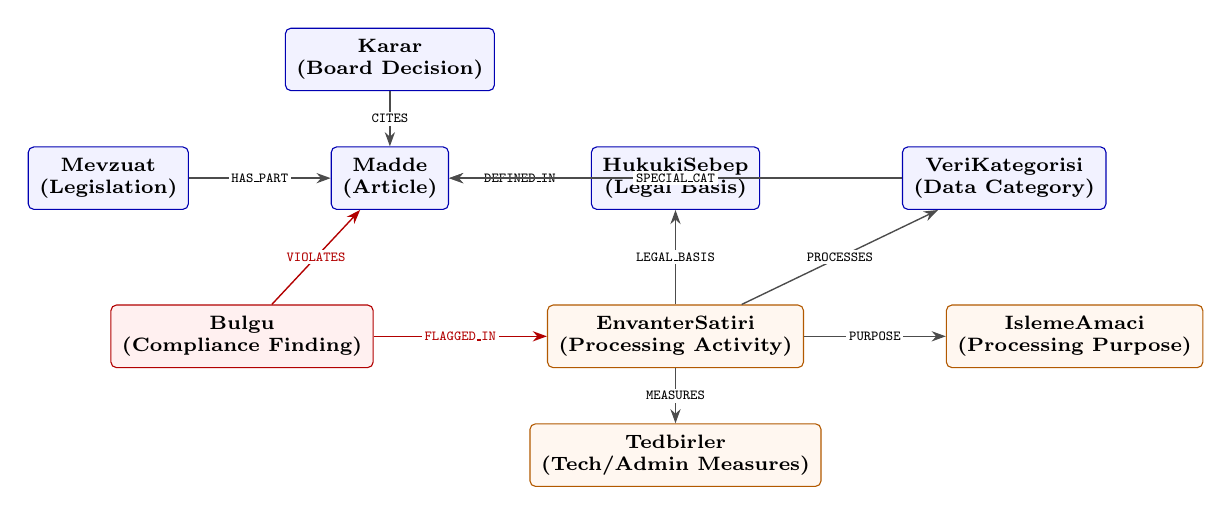
\begin{tikzpicture}[
  law/.style={draw=blue!70!black, fill=blue!5, rounded corners=2pt, font=\scriptsize\bfseries, align=center, inner sep=4pt},
  inv/.style={draw=orange!70!black, fill=orange!6, rounded corners=2pt, font=\scriptsize\bfseries, align=center, inner sep=4pt},
  audit/.style={draw=red!70!black, fill=red!6, rounded corners=2pt, font=\scriptsize\bfseries, align=center, inner sep=4pt},
  edge_lbl/.style={font=\tiny, fill=white, inner sep=1pt},
  arrow/.style={-{Stealth[length=1.8mm, width=1.3mm]}, line width=0.5pt, draw=black!70}
]

  % Legal Layer (Top)
  \node[law] (mev) {Mevzuat\\(Legislation)};
  \node[law, right=1.8cm of mev] (madde) {Madde\\(Article)};
  \node[law, above=0.7cm of madde] (karar) {Karar\\(Board Decision)};
  \node[law, right=1.8cm of madde] (hsebep) {HukukiSebep\\(Legal Basis)};
  \node[law, right=1.8cm of hsebep] (vkat) {VeriKategorisi\\(Data Category)};

  \draw[arrow] (mev) -- node[edge_lbl]{\texttt{HAS\_PART}} (madde);
  \draw[arrow] (karar) -- node[edge_lbl]{\texttt{CITES}} (madde);
  \draw[arrow] (hsebep) -- node[edge_lbl]{\texttt{DEFINED\_IN}} (madde);
  \draw[arrow] (vkat) -- node[edge_lbl]{\texttt{SPECIAL\_CAT}} (madde);

  % Inventory & Compliance Layer (Bottom)
  \node[inv, below=1.2cm of hsebep] (env) {EnvanterSatiri\\(Processing Activity)};
  \node[inv, right=1.8cm of env] (amac) {IslemeAmaci\\(Processing Purpose)};
  \node[inv, below=0.7cm of env] (tedbir) {Tedbirler\\(Tech/Admin Measures)};
  \node[audit, left=2.2cm of env] (bulgu) {Bulgu\\(Compliance Finding)};

  \draw[arrow] (env) -- node[edge_lbl]{\texttt{LEGAL\_BASIS}} (hsebep);
  \draw[arrow] (env) -- node[edge_lbl]{\texttt{PROCESSES}} (vkat);
  \draw[arrow] (env) -- node[edge_lbl]{\texttt{PURPOSE}} (amac);
  \draw[arrow] (env) -- node[edge_lbl]{\texttt{MEASURES}} (tedbir);

  \draw[arrow, draw=red!70!black] (bulgu) -- node[edge_lbl, text=red!70!black]{\texttt{FLAGGED\_IN}} (env);
  \draw[arrow, draw=red!70!black] (bulgu) -- node[edge_lbl, text=red!70!black]{\texttt{VIOLATES}} (madde);

\end{tikzpicture}
\caption{Knowledge graph schema linking statutory provisions to operational inventory activities. 13 node types and 13 edge types connect formal legislation and official decisions to enterprise processing records and automated compliance audit findings.}
\label{fig:graph}
\end{figure*}

%%% ====================================================================
%%% 6. DISCUSSION
%%% ====================================================================
\section{Discussion}
\label{sec:discussion}

\subsection{Structure-Aware Chunking Outperforms Fixed-Length Chunking on Legal Text}

Structure-aware chunking raised the mean MRR by 45\% over the recursive baseline (0.167 $\rightarrow$ 0.242) and lifted the best R@10 from 0.34 to 0.51. This goes \textbf{against} the finding of Qu et al.~\cite{qu2025}, who report that fixed-size chunking consistently outperforms semantic chunking.

But we think this is not a real contradiction. Qu et al. evaluate statistical semantic chunking (embedding-similarity breakpoints) on general-domain prose. Our approach is different: for legislation, we parse an explicit, author-provided hierarchy (\texttt{MADDE n}). This is not an estimate of where a topic boundary might be --- it is a declaration by the law's author. The semantic component only applies to the decision corpus, where no such markup exists.

So the correct reading of our result is: \textbf{where a document declares its own structure, use it}. Qu et al.'s caution against paying for inferred boundaries is still valid.

\subsection{Provenance Prefix Effect}

Isolating the provenance prefix effect (\texttt{recursive} $\rightarrow$ \texttt{recursive+prefix}, same boundaries) raised mean MRR from 0.167 to 0.200 (+20\%). The effect is very concentrated:

\begin{itemize}[leftmargin=*]
  \item BERTurk@75 dense R@1 went from 0.03 to 0.14 --- a 4.7$\times$ gain from adding just ${\sim}$60 characters of prefix.
  \item BM25 Recall@5 on referential queries doubled (0.20 $\rightarrow$ 0.40).
\end{itemize}

This is basically a free, deterministic, LLM-free version of Contextual Retrieval~\cite{anthropic2024}, and it gives a similar benefit at zero cost. The reason is clear from the query-type analysis: the prefix is the only place where the article or decision identifier appears as searchable text.

\textbf{Important design lesson.} The lexical index must cover the prefixed text, not the raw body. Our first implementation indexed \texttt{text\_raw} (without prefix), which silently made every referential query unanswerable by BM25. We only found this through the query-type disaggregation. This is the strongest argument in this study for always reporting metrics by query class.

\subsection{The Truncating Encoder Problem}

\texttt{emrecan/bert-base-turkish-cased-mean-nli-stsb-tr} ships with \texttt{max\_seq\_length\,=\,75} even though the BERT backbone supports 512 positions. We measured this directly: the embedding of a 1,320-character chunk and that of its first 300 characters have cosine similarity \textbf{1.0000}. Everything after the 75th token is simply thrown away, with no warning and no exception. Under recursive chunking (median 970 characters), about three-quarters of every chunk was invisible to the retriever, which explains the R@1 of 0.03.

Setting \texttt{max\_seq\_length} to 512 removed the truncation, but it \textbf{did not reliably improve retrieval}. In the structural+semantic arm, dense R@10 actually got worse (0.46 $\rightarrow$ 0.40). The reason is that reading more tokens is not the same as understanding them well. The model was fine-tuned on short NLI/STS pairs, and making it process 512 tokens moves it outside its training distribution. Mean pooling over many weakly-modeled tokens dilutes the signal from the first 75 tokens.

The practical lesson is general: \textbf{\texttt{max\_seq\_length} must be verified empirically}, not assumed from the backbone architecture. This type of defect is completely invisible --- no error, no warning, and the neighbors still look plausible.

\subsection{Hybrid Fusion Is Conditional}

Hybrid retrieval has the best marginal mean MRR (0.225), but the aggregate number hides an important interaction:

\begin{table}[t]
\centering
\caption{Hybrid fusion effect depends on dense encoder quality (structural+semantic chunking).}
\label{tab:fusion}
\small
\begin{tabular}{@{}lccc@{}}
\toprule
\textbf{Dense quality} & \textbf{Dense} & \textbf{Hybrid} & $\boldsymbol{\Delta}$ \\
\midrule
Weak (berturk@75) & 0.172 & 0.305 & \textbf{+77\%} \\
Strong (e5-base)  & 0.330 & 0.292 & \textbf{--12\%} \\
\bottomrule
\end{tabular}
\end{table}

With a fixed fusion constant (RRF, $k{=}60$), BM25 contributes the same amount regardless of whether the dense ranking actually needs help. When the dense retriever is already strong, fusion injects a weaker ranking and makes the result worse. The best single configuration by MRR (\texttt{structural+semantic} $\times$ \texttt{e5-base} $\times$ \texttt{dense}, 0.330) uses no fusion at all.

This qualifies the common belief that ``hybrid is always better.'' A better production choice would be adaptive fusion --- weighting BM25 by dense-score confidence, or routing referential queries to the lexical index and conceptual queries to the dense index.

\subsection{The Remaining Gap}

Without reranking, the production pipeline failed on 10 of 35 questions (R@10\,=\,0.71). With cross-encoder reranking and recalibrated authority weighting ($w{=}2.0$), we reached \textbf{R@10\,=\,0.77} (8~misses) and \textbf{MRR\,=\,0.657} --- a 73\% improvement over un-reranked hybrid.

The remaining 8 misses reflect cases where neither the bi-encoder's semantic similarity nor the cross-encoder's token interactions can bridge the vocabulary gap between the user's everyday language and the law's formal terminology, without explicit domain knowledge.

Following the recommendation of RAGTurk~\cite{ragturk2026} that stacking generative modules distorts Turkish morphological cues, the next steps should be:

\begin{enumerate}[leftmargin=*]
  \item Deterministic query expansion from a curated legal-terminology synonym map (e.g., \textit{parmak izi} $\rightarrow$ \textit{biyometrik veri}), which directly attacks the vocabulary misses without a generative stage.
  \item Knowledge graph integration (Figure~\ref{fig:graph}) to link regulatory articles with concrete data categories. The graph schema already connects 13 node types across legislation, inventory, and compliance findings to support structured compliance queries.
\end{enumerate}

\subsection{Corpus Composition as a Retrieval Problem}

Decision summaries are 87\% of the corpus but the second-lowest authority class. Pure similarity retrieval reflects this imbalance faithfully and therefore wrongly: for the question ``can I install a fingerprint reader at the office entrance?'', the unweighted retriever returned ten advisory summaries and \textbf{zero binding provisions}. The generated answer was fluent and well-structured but cited only non-binding sources.

Neither a post-hoc quota nor score weighting fully fixes this. A quota can only promote candidates that are already in the pool, and the relevant article (Article~6) never entered it. The effective remedy is a \textbf{separate metadata-filtered retrieval pass} over the binding subset. Grounding is thus an index-design requirement, not a prompt instruction.

\subsection{Threats to Validity}

\textbf{Gold set size.} 35 questions, of which only 5 are referential. Referential recall therefore moves in steps of 0.20, making the query-type comparison indicative rather than conclusive.

\textbf{Single annotator.} The gold set was authored by one annotator and verified only for resolvability, not for inter-annotator agreement. Some questions may have more than one defensible answer.

\textbf{No statistical testing.} With 35 questions, small differences (0.02--0.03) could be sampling noise. The chunking effect (+45\% mean MRR) is large enough to survive this caveat; the embedding and fusion effects should be read as directional.

\textbf{Retrieval only.} We do not measure answer-generation quality. As Abualhaija et al.~\cite{abualhaija2025} show, retrieval success and citation groundedness can diverge.

%%% ====================================================================
%%% 7. ADOPTED CONFIGURATION
%%% ====================================================================
\section{Adopted Configuration}
\label{sec:config}

Based on all the results, we adopted the configuration shown in Table~\ref{tab:adopted}.

\begin{table}[t]
\centering
\caption{Production configuration with the section that justifies each choice.}
\label{tab:adopted}
\small
\begin{tabular}{@{}llc@{}}
\toprule
\textbf{Component} & \textbf{Setting} & \textbf{Ref.} \\
\midrule
Chunking        & structural + semantic    & §\ref{sec:discussion}.1 \\
Prov. prefix    & on (both indices)        & §\ref{sec:discussion}.2 \\
Embedding       & e5-base, 512 tok.        & §\ref{sec:discussion}.3 \\
Retrieval       & hybrid RRF ($k{=}60$)    & §\ref{sec:discussion}.4 \\
Mandatory pass  & top-10, binding only     & §\ref{sec:discussion}.6 \\
Reranker        & bge-reranker-v2-m3       & §\ref{subsec:sigmoid} \\
Authority $w$   & 2.0                      & §\ref{subsec:auth_results} \\
Returned units  & 12 parents               & §\ref{subsec:retrieval} \\
\bottomrule
\end{tabular}
\end{table}

End-to-end retrieval quality: \textbf{R@10\,=\,0.77, R@5\,=\,0.71, R@1\,=\,0.60, MRR\,=\,0.657, nDCG\,=\,0.684}, 8 of 35 questions unretrieved, 0 questions without a binding source. Query latency is 0.60~seconds with both encoders on GPU, peak VRAM 2.59~GB.


%%% ====================================================================
%%% 8. CONCLUSION
%%% ====================================================================
\section{Conclusion}
\label{sec:conclusion}

In this study, we evaluated how chunking strategy, embedding model, and retrieval mode interact on a Turkish legal corpus for retrieval-augmented generation. Our main findings are:

\begin{enumerate}[leftmargin=*]
  \item \textbf{Chunking strategy is the most important factor}, not the embedding model. Structure-aware chunking gave +45\% mean MRR improvement over the recursive baseline. This contradicts the general finding that fixed-size chunking outperforms semantic chunking, but the difference is that we use explicit document structure rather than statistical boundary inference.

  \item \textbf{The biggest single improvement came from authority weighting} (+30\% MRR without reranking, +73\% with), which is a domain-specific ranking signal that does not appear in general RAG guidance.

  \item \textbf{The most dangerous defects were silent}: an encoder that discards three-quarters of every chunk without any error, and a default sigmoid that collapses cross-encoder logits into near-zero variance. Both were only detectable by direct, component-isolated measurement.

  \item \textbf{Hybrid retrieval is not universally better}. When the dense encoder is already strong, adding BM25 with a fixed fusion weight can actually degrade results. Adaptive fusion or query-type routing would be a better approach.
\end{enumerate}

The final system retrieves a correct binding source for roughly eight of ten questions (R@10\,=\,0.77, MRR\,=\,0.657) and always returns at least one binding provision. This represents a reliable basis for a compliance assistant. The remaining frontier lies in bridging domain-specific vocabulary gaps through deterministic query expansion and integrating structured knowledge.


%%% ====================================================================
%%% REFERENCES
%%% ====================================================================
\bibliographystyle{plain}

\begin{thebibliography}{9}

\bibitem{qu2025}
R.~Qu, R.~Tu, and F.~Bao,
``Is semantic chunking worth the computational cost?''
\textit{Findings of NAACL}, pp.~2155--2177, 2025.
arXiv:2410.13070.

\bibitem{jurix2024}
``Legal chunking: Evaluating methods for effective legal text retrieval,''
\textit{JURIX 2024, Frontiers in Artificial Intelligence and Applications},
DOI:~10.3233/FAIA241255.

\bibitem{ragturk2026}
Ünlü et al.,
``RAGTurk: Best practices for retrieval augmented generation in Turkish,''
\textit{SIGTURK 2026}.
arXiv:2602.03652.

\bibitem{turkel2026}
M.~S.~Türkel, F.~N.~Korkmaz, and A.~T.~Bayrak,
``Comparing chunking and embedding strategies for Turkish RAG systems,''
\textit{INTCEC 2026}.
arXiv:2608.26192.

\bibitem{abualhaija2025}
S.~Abualhaija, M.~Ceci, N.~Sannier, D.~Bianculli, S.~Lannier, M.~Siclari,
O.~Voordeckers, and S.~Tosza,
``LLM-assisted extraction of regulatory requirements: A case study on the GDPR,''
\textit{RE 2025}.

\bibitem{gunther2024}
M.~Günther et al.,
``Late chunking: Contextual chunk embeddings using long-context embedding models,''
2024.

\bibitem{anthropic2024}
Anthropic,
``Introducing contextual retrieval,''
2024.

\bibitem{lewis2020}
P.~Lewis et al.,
``Retrieval-augmented generation for knowledge-intensive NLP tasks,''
\textit{NeurIPS 2020}.

\end{thebibliography}

\end{document}
